\chapter{$\mu$-演算中的遗忘理论}
\label{chapter06}

{\em 本章探索$\mu$-演算中的遗忘理论。$\mu$-演算是描述转换系统性质重要逻辑语言,其具有表达能力强的优点:$\mu$-演算是一种表达能力与S2S\footnote{无限完全二叉树下的一元二阶理论(monadic second order theory of the infinite complete binary tree),简称为S2S。}相同的逻辑语言,LTL(线性时序逻辑,linear temporal logic)、CLT和CTL$^*$能表达的属性都能用$\mu$-演算来表示。
	
	已有研究表明$\mu$-演算具有均匀插值性质,这体现了$\mu$-演算下的遗忘理论研究本质上与$\CTL$下的不同。本章首先给出$\mu$-演算下的遗忘理论的定义。其次,表明$\mu$-演算下的遗忘理论是封闭的,这是其与$\CTL$下的遗忘理论的最大的不同。最后,模型检测问题作为形式化验证的重要方法,本章给出$\mu$-演算下遗忘理论的模型检测和推理问题的复杂性结果。
	}

\section{引言}
$\mu$-演算是一种表达能力较强的语言,它能表达$\CTL$不能表示的性质,例如:Kripke结构中有一条路径,在这条路径上的基数状态满足公式$\neg q \wedge \neg p$,但是偶数状态满足$q \wedge p$。这一性质是不能用$\CTL$公式来表示,但是可以用$\mu$-演算公式表示如下:
$$\varphi = \nu X.(p \wedge q) \wedge \EXIST \NEXT(\neg p \wedge \neg q) \wedge \EXIST \NEXT \EXIST \NEXT X.$$

这种情形在日常生活中是很常见的,如:偏序关系$(N, \leq)$(自然数集上的小于等于关系)构成的Kripke结构,其基数节点为基数、偶数节点为偶数。
事实上,$\CTL$不能表达具有有规则的性质~\cite{DBLP:journals/iandc/Wolper83},其主要原因是
\begin{quote}
	\emph{Given a proposition $p$, any proposinal temporal formula (PTL) $f(p)$ containing 
	n ``next" ($\NEXT$) operators has the same truth value on all sequences of the form 
	$p^i(\neg p) p^w$, $i > n$.}
\end{quote}

因而得出如下结论:
\begin{quote}
	\emph{For any given $m\geq 2$, the property ``$p$ is true in every 
	state $s_i$, where $i = km$ (integer $k\geq 0$)" is not expressible in PTL.}
\end{quote}



均匀插值是一个重要的逻辑概念,其有以下含义:给定两个具有$\varphi\models\psi$关系的公式$\varphi$和$\psi$,如果存在公式$\theta$使得$\varphi\models \theta$、$\theta \models \psi$且$\Var(\theta) \subseteq \Var(\varphi) \cap \Var(\psi)$,则称公式$\theta$是$\varphi$和$\psi$的Craig插值。若$\theta$与$\psi$无关,而只与$\Var(\varphi) \cap \Var(\psi)$有关,则称$\theta$为$\varphi$关于$\Var(\varphi) \cap \Var(\psi)$的均匀插值。
均匀插值的定义~\cite{d2006modal}如下(注意:这里的$\Var(\varphi)$表示出现在$\varphi$中的原子命题和变元的集合):                                                                                                                                                                                                                                              
\begin{definition}
	给定一个$\mu$-句子$\varphi$和原子命题的集合$V$,$\varphi$关于$V$的均匀插值是满足下列条件的$\mu$-句子$\theta$:
	\begin{itemize}
		\item $\varphi \models \theta$;
		\item 对任意的公式$\psi$,若$\Var(\varphi) \cap \Var(\psi)\subseteq V$,则$\varphi \models \psi$;
		\item $\Var(\theta) \subseteq V$。 
	\end{itemize}
\end{definition}


从直观上来说,$\varphi$关于$\Var(\varphi) \cap \Var(\psi)$的均匀插值是从$\varphi$中“移除”掉不在$\Var(\varphi) \cap \Var(\psi)$中的原子命题而保留其在$\Var(\varphi) \cap \Var(\psi)$上的结论得到的结果。这与遗忘有着密切的关系。

再者,在背景知识部分已经指出,任意的$\mu$-演算公式都能转换成吸取$\mu$-公式,在这种形式下的公式的均匀插值是容易计算的,即:
\begin{theorem}[定理 3.6~\cite{d2006modal}]
	吸取$\mu$-公式$\varphi$的均匀插值$\exists p \varphi$与$\mu$-公式$\varphi[p/\top, \neg p/ \bot]$等价,其中$\varphi[p/\top, \neg p/ \bot]$是同时将$p$及其否定$\neg p$分别用$\top$和$\bot$替换得到。
\end{theorem}



尽管上面的定义中使用的$\Var(\varphi)$表示出现在$\varphi$中的原子命题和变元的集合,但是均匀插值指的是与原子命题相关的部分,即:对任意的$\mu$-句子$\varphi$和原子命题$p$,存在一个$\mu$-句子$\widetilde{\exists} p. \varphi$使得$\widetilde{\exists} p. \varphi$是$\varphi$关于$\{p\}$的一个均匀插值。这表明在讨论均匀插值时,不考虑变元,即:不是$\varphi$关于某个变元的均匀插值。%实际上,$\mu$-句子里的变元都是受约束的变元。

本章将要说明本文所定义的$\mu$-演算下的遗忘与~\cite{d2006modal}中定义的均匀插值是一对对偶概念,此时本文给出的遗忘的性质无疑也是均匀插值所具有的性质,这为$\mu$-演算的均匀插值的探索提供了另一种思路。此外,借助于均匀插值的计算方法,本文也给出了计算遗忘的方法。这形成了遗忘和均匀插值之间相辅相成的作用。

本章的组织结构如下。首先,给出$\mu$-演算下遗忘的定义;然后,探讨遗忘的一般性质,并给出其与均匀插值的关系;最后给出与遗忘相关的问题的复杂性。

\section{遗忘的定义}\label{sec:chapter06-system-model}
与$\CTL$情形下的遗忘相似,这里先给出$V$互模拟的定义。不失一般性地,令$\Hm_i = (S_i, r_i, R_i, L_i)$,$i$为自然数集$\mathbb{N}$中的元素。
\begin{definition}[$V$-互模拟]\label{def:VB}
	给定原子命题集合$V \subseteq \Ha$和两个Kripke结构$\Hm_1$ 和 $\Hm_2$。若下面几个条件满足,则称$\Hb\subseteq S_1 \times S_2$是$\Hm_1$ 和 $\Hm_2$的$V$-互模拟关系:
	\begin{itemize}
		\item $r_1 \Hb r_2$,
		\item 对任意的$s\in S_1$ 和 $t\in S_2$,若$s \Hb t$ 则对任意的$p \in \Ha- V$有 $p \in L_1(s)$ 当且仅当 $p \in L_2(t)$,
		\item $(s, s')\in R_1$ 和 $s \Hb t$蕴涵存在一个 $t'$ 使得 $s' \Hb t'$ 和 $(t, t')\in R_2$,且
		\item 若 $s \Hb t$ 且 $(t, t')\in R_2$,则存在一个$s'$ 使得 $(s, s')\in R_1$ 和 $t' \Hb s'$。
	\end{itemize}
\end{definition}

与$\CTL$下的$V$-互模拟不同的是,这里要求$r_1 \Hb r_2$(即:$(r_1,r_2)\in \Hb$)。
如果$\Hm_1$ and $\Hm_2$之间存在一个$V$-互模拟关系${\cal B}$则称这两个Kripke结构$\Hm_1$ 和 $\Hm_2$是$V$-互模拟的,记为$\Hm_1 \lrto_V \Hm_2$,
%In this case, $\Hm_1$ and $\Hm_2$ are bisimilar on $V$.
\begin{example}
	如图~\ref{chapter06:fig:bisim}中的两个Kripke结构$\Hm=(S,r,R,L)$ 和 $\Hm'=(S',r',R',L')$,其中:
	\begin{itemize}
		\item $S=\{s_0,s_1,s_2\}$,$S'=\{t_0,t_1\}$,$r=s_0$,$r'=t_0$;
		\item $R=\{(s_0,s_1),(s_1,s_0),(s_0,s_2),(s_2,s_0)\}$,$R'=\{t_0,t_1\}$;
		\item $L(s_0)=\{ch,j\}$,$L(s_1)=L(s_2)=\emptyset$,$L'(t_0)=\{j\}$,$L'(t_1)=\emptyset$。
	\end{itemize}
	由于$\Hm$ 和 $\Hm'$之间存在一个二元$\{ch\}$-互模拟$\Hb=\{(s_0, t_0), (s_1, t_1), (s_2, t_1)\}$ $\Hm \lrto_{\{ch\}} \Hm'$,所以$\Hm\lrto \Hm'$。
	
	
	
	% 	\begin{center}\label{fig:bisim}
	% 		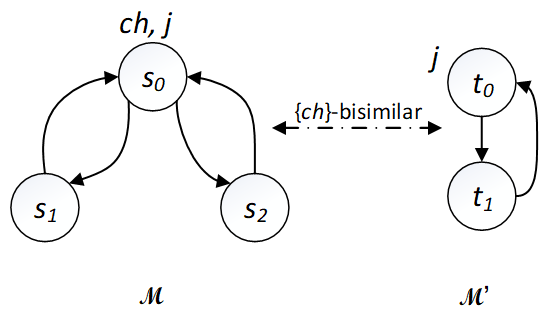
\includegraphics[width=5cm,height=3cm]{chBisimilar.png}\\
	% 		%\vspace{2mm}
	% 		\parbox[c]{7cm}{\textbf{Fig.1~}  Two $\{ch\}$-bisimilar Kripke structures}%\vspace*{.2mm}
	% 	\end{center}
	
	\begin{figure}[h]%
		\centering
		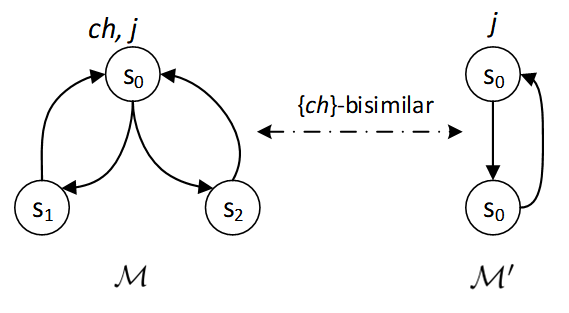
\includegraphics[width=4.5cm,height=2.5cm]{chapter06/chvB.png}
		\caption{两个 $\{ch\}$-互模拟的Kripke结构}\label{chapter06:fig:bisim}
		
		% $s_0$ is labeled by $\{ch, j\}$, $t_0$ is labeled by $\{j\}$, and $s_1$, $s_2$, and $t_1$ are labeled by $\emptyset$.}\label{fig:bisim}
	\end{figure}
	
\end{example}

可以容易证明$\lrto_V$为一个等价关系,此外还有如下性质。

\begin{proposition} \label{pro:EqUnion}
	令$V, V_1 \subseteq \Ha$为原子命题的集合,$\Hm_1$、 $\Hm_2$ 、 $\Hm_3$为Kripke 结构,则:
	\begin{itemize} 
		\item[(i)] $\lrto_V$ 是 Kripke 结构之间的等价关系;
		\item[(ii)] 若 $\Hm_1 \lrto_V \Hm_2$ 且 $\Hm_2 \lrto_{V_1} \Hm_3$,则 $\Hm_1 \lrto_{V \cup V_1} \Hm_3$。
	\end{itemize}
	
\end{proposition}
\begin{proof}
	(i) 这里从自反性、对称性和传递性来证明该关系是一个等价关系。
	
	(1) $\lrto_V$是自反的。容易检查对任意的Kripke结构$\Hm$都有$\Hm\lrto_V \Hm$。
	
	(2) $\lrto_V$ 是对称的。 这里证明对任意的$\Hm_1$ 和 $\Hm_2$,若 $\Hm_1 \lrto_V \Hm_2$ 则 $\Hm_2 \lrto_V \Hm_1$。
	$\Hm_1$和 $\Hm_2$之间存在$V$-互模拟关系$\Hb$,构造如下二元关系$\Hb_1=\{(s,t) \mid (t, s)\in \Hb\}$,现在从下面几点证明$\Hb_1$是$\Hm_2$ 和 $\Hm_1$ 之间的一个$V$-关系:
	\begin{itemize}
		\item 由于$r_1 \Hb r_2$,所以 $r_2 \Hb_1 r_1$,
		\item 对任意的$s\in S_1$ 和 $t\in S_2$,若 $t \Hb_1 s$,则 $s\Hb t$,因此对于任意的$p \in \Ha - V$,$p \in L_1(s)$ 当且仅当 $p \in L_2(t)$,且
		\item 因为$\Hb$是$\Hm_1$和 $\Hm_2$之间存在$V$-互模拟关系,所以$V$-互模拟的第三和第四个点很容易能够证明。
	\end{itemize}
	
	(3) $\lrto_V$是传递的。这里证明对任意的 $\Hm_1$、$\Hm_2$、和 $\Hm_3$,若 $\Hm_1 \lrto_V \Hm_2$ 和 $\Hm_2 \lrto_V \Hm_3$则 $\Hm_1 \lrto_V \Hm_3$。 假定$\Hm_1$和 $\Hm_2$之间存在$V$-互模拟关系为$\Hb_1$,$\Hm_2$和 $\Hm_3$之间存在$V$-互模拟关系$\Hb_2$,构造二元关系: $\Hb=\{(s, z) \mid (s,t) \in \Hb_1,\ (t, z)\in \Hb_2\}$。
	此时,可以像(2)一样证明 $\Hb$ 是$\Hm_1$ 和 $\Hm_3$之间的一个 $V$-互模拟关系。因此,$\Hm_1 \lrto_V \Hm_3$。
	
	(ii) 为了证明$\Hm_1 \lrto_{V\cup V_1} \Hm_3$,只需找到一个  $\Hm_1$ 和 $\Hm_3$之间的二元$(V\cup V_1)$-互模拟关系$\Hb$。
	假定$\Hm_1$和 $\Hm_2$之间存在$V$-互模拟关系为$\Hb_1$,$\Hm_2$和 $\Hm_3$之间存在$V_1$-互模拟关系$\Hb_2$。令$\Hb = \{(s_1, s_3)\mid (s_1, s_2) \in \Hb_1, \ (s_2, s_3) \in \Hb_2\}$,容易证明$\Hb$是$\Hm_1$ 和 $\Hm_3$之间的二元$(V\cup V_1)$-互模拟关系。
\end{proof}

直观地说,(i)表示$\lrto_V$是Kripke结构的集合上的自反、对称和传递关系。
(ii)表示如果一个Kripke结构和其他两个Kripke结构互相$V$和$V_1$互模拟,则这两个Kripke结构$V\cup V_1$-互模拟。这跟$\CTL$情形下的互模拟类似,正如下文将要说到的那样,这一性质有助于证明$\mu$-演算下遗忘的模块属性。

此时,$\mu$-演算下的遗忘如下定义:
\begin{definition}[$\mu$-演算下的遗忘]\label{chapter06:def:V:forgetting}
	令$V\subseteq\cal A$ 和 $\phi$ 为$\mu$-句子。若下面等式成立,则称
	$V$上的 $\mu$-句子 $\psi$是从$\phi$中遗忘掉$V$后得到的结果,记为 $\Muforget(\phi, V)$:
	\begin{equation*}
		\Mod(\psi)=\{\Hm  \mid \exists \Hm' \in\Mod(\phi)\ \&\ \Hm' \lrto_V \Hm\}.
	\end{equation*}
\end{definition}

定义~\ref{chapter06:def:V:forgetting}表明如果 $\psi$ 和 $\psi'$ 都是从$\phi$中遗忘掉 $V$ 中的原子命题得到的结果,则
$\Mod(\psi)=\Mod(\psi')$,也就是说遗忘的结果之间是语义等价的(即有相同的模型)。
%, i.e., $\psi$ and $\psi'$ have the same models. 


D'Agostino 研究了 $\mu$-演算下的均匀插值,并指出 $\mu$-算具有均匀插值性质~\cite{d1996uniform,d2000logical,d2006modal}。换句话说,这意味着对任意的 $\mu$-句子 $\varphi$ 和有限的原子命题的集合$V\subseteq \Var(\varphi)$,都存在一个$V$-无关且与$\varphi$最接近的 $\mu$-句子 $\widetilde{\exists}V \varphi$。
值得注意的是,上述定义的遗忘 $\Muforget(\phi, V)$与 $\widetilde{\exists}V \varphi$~\cite{d2006modal}语义等价.

\section{遗忘的一般属性}
这部分展示$\mu$-演算下遗忘的语义属性。特别地,这里将证明上述$\mu$-演算下的遗忘的定义与遗忘的那几条规则具有“当且仅当的关系”,且从任意$\mu$-句子中遗忘掉任意原子命题的集合的结果总是一个$\mu$-句子。此外,也研究了遗忘算子的代数属性,包括模块性(modularity)、交换性(commutativity)和同质性(homogeneity)。

\begin{theorem} \label{thm:exist}
	给定原子命题 $q \in \cal A$ 和$\mu$-句子 $\phi$,则存在一个$\mu$-句子 $\psi$ 使得 $\IR(\psi, \{q\})$ 且 $\psi \equiv \Muforget(\phi, \{q\})$。
\end{theorem}
\begin{proof}
	已有结果表明,对任意的$\mu$-句子$\phi$和和原子命题$p$,存在一个$\{p\}$-无关的$\mu$-句子$\phi'$(即$\IR(\phi', \{p\})$)使得(定理 3.1 \cite{d1996uniform}):
		\[
	\Hm \models \phi' \mbox{ 当且仅当 } \exists \Hm' \in \phi \mbox{ 使得 } \Hm \lrto_{\{p\}} \Hm'.
	\]
	
	这与本文遗忘的定义一致,因此上述结论成立。
\end{proof}

与模态S5和$\CTL$情形类似,下面给出$\mu$-演算下的遗忘的基本准则:
\begin{itemize}
	\item[(\W)]  削弱(Weakening): $\varphi \models \varphi'$;
	\item[(\PP)]  正支持 (Positive Persistence):
	对任意的$\mu$-句子 $\eta$,若$\IR(\eta, V)$ 和 $\varphi \models \eta$ 则 $\varphi' \models \eta$;
	\item[(\NgP)]  负支持(Negative Persistence):对任意的 $\mu$-句子$\eta$,若$\IR(\eta, V)$ 和 $\varphi \not \models \eta$ 则 $\varphi' \not \models \eta$;
	\item[(\textbf{IR})]  无关性(Irrelevance): $\IR(\varphi', V)$。
\end{itemize}
其中 $V\subseteq\cal A$、
$\varphi$ 为$\mu$-句子 、 $\varphi'$ 是 从$\varphi$中遗忘掉$V$后得到的结果。

\begin{theorem}[表达性定理]\label{chapter06:thm:Rep}
	给定$\mu$-句子 $\varphi$、 $\varphi'$ 和 $\phi$, $V \subseteq \Ha$为原子命题的集合。
	下面的几个陈述是等价的:
	\begin{itemize}
		\item[(i)] $\varphi' \equiv \Muforget(\varphi, V)$,
		\item[(ii)] $\varphi'\equiv \{\phi \mid\varphi \models \phi \text{ 且 } \IR(\phi, V)\}$,
		\item[(iii)] 若$\varphi$、 $\varphi'$ 及 $V$和(i)、(ii)中的符号表示相同公式和原子命题的集合,则 (\W)、 (\PP)、 (\NgP) 和 (\textbf{IR}) 成立。
	\end{itemize}
\end{theorem}
\begin{proof}
	$(i) \LRto (ii)$. 为了证明这一结论成立,只需证明:
	\[
	\Mod(\Muforget(\varphi, V)) = \Mod(\{\phi \mid \varphi \models \phi, \IR(\phi, V)\}).\]
	$(\Rto)$ 对$\Muforget(\varphi, V)$的任意模型 $\Hm'$ \\
	$\Rto$  $\exists\Hm$ 使得 $\Hm \models \varphi$ 和 $\Hm \lrto_V \Hm'$ \hfill (定义~\ref{chapter06:def:V:forgetting}) \\
	$\Rto$ 对于任意与$V$-无关且$\varphi \models \phi$的$\phi$ 都有 $\Hm' \models \phi$ \\
	$\Rto$ $\Hm' \models \{\phi \mid \varphi \models \phi, \IR(\phi, V)\}$
	
	$(\Lto)$ 由于$\IR(\Muforget(\varphi, V),V)$和$\varphi \models \Muforget(\varphi, V)$,由定义~\ref{chapter06:def:V:forgetting}可知 $\{\phi \mid \varphi \models \phi, \IR(\phi, V)\} \models \Muforget(\varphi, V)$。
	
	$(ii) \Rto (iii)$. 为了方便,令$A = \{\phi \mid \varphi \models \phi, \IR(\phi, V)\}$。
	首先,对任意的$A$中的公式$\phi'$都有$\IR(\phi',V)$,所以有$\IR(A,V)$。
	因此,$\IR(\varphi', V)$。 其次,对任意的 $\phi'\in A$,都有$\varphi \models \phi'$,所以$\varphi \models \varphi'$。
	%The (\NgP) and (\PP) are obvious from $A$.
	第三, $\forall \phi$ 且$\IR(\phi, V)$,若$\varphi \models \phi$ 则 $\phi \in A$,因而$\varphi' \models \phi$。
最后, $\forall \phi$ 且 $\IR(\phi, V)$,若 $\varphi \not \models \phi$ 则 $\phi \not \in A$。因此,由定义~\ref{chapter06:def:V:forgetting}和$V$-无关性可知$\varphi' \not \models \phi$。
	
	$(iii) \Rto (ii)$. (1) $\varphi' \models \{\phi \mid \varphi \models \phi, \IR(\phi, V)\}$  \hfill ((\PP))\\
	(2) $\{\phi \mid \varphi \models \phi, \IR(\phi, V)\} \models \varphi'$ \hfill ((\W), (\textbf{IR}))\\
	$\Rto$ $\varphi'\equiv \{\phi \mid\varphi \models \phi, \IR(\phi, V)\}$ \hfill ((1), (2)).
\end{proof}


定理~\ref{chapter06:thm:Rep} 表明$\mu$-演算下的遗忘跟其基本准则形成了一个“当且仅当”的关系:基本准则能描述遗忘的结果,遗忘的结果具有基本准则里的性质。这与S5和$\CTL$下的情形相同。

除了上述的表达性定理,后文将说明准则(\textbf{IR})对计算SNC 和 WSC是重要的。对于$\mu$-句子$\psi = \varphi \wedge (q \lrto \alpha)$,$\varphi \wedge \alpha$ 是 $\{q\}$-无关的,则从$\psi$中遗忘掉 $q$得到的结果是$\varphi$。正如将在第~\ref{chapter07}中展示,这一性质有助于将任意公式的SNC(WSC)转换为命题下的SNC(WSC)。这一性质可形式化如下:

\begin{lemma}
	\label{lem:KF:eq}
	令 $\varphi$ 和 $\alpha$为两个 $\mu$-句子,$q$为原子命题且 $q \not \in  \Var(\varphi) \cup \Var(\alpha)$。则
	$\Muforget(\varphi \wedge (q\lrto\alpha), q)\equiv \varphi$。
\end{lemma}
 \begin{proof}
	令 $\varphi' =\varphi \wedge (q\lrto\alpha)$。对$\Muforget(\varphi', q)$的任意一个模型${\cal M}$,存在一个Kripke结构 ${\cal M}'$使得 ${\cal M}\lrto_{\{q\}}{\cal M}'$ 和 ${\cal M}' \models \varphi'$。显然有 ${\cal M}' \models \varphi$,又因为$\IR(\varphi,\{q\})$ 和 ${\cal M} \lrto_{\{q\}} {\cal M}'$,所以 ${\cal M} \models \varphi$。
	%	by the invariant of $\mu$-sentence for $\overline{V}$-bisimulation~\cite{d1996uniform}.
	
	令 $\Hm \in \Mod(\varphi)$, 其中 ${\cal M}=(S, s, R, L)$。如下构造 $\Hm' = (S, s, R, L')$:
	\begin{align*}
		& L':S \rto 2^{\Ha}\ and\ \forall s^*\in S, L'(s^*) = L(s^*) - \{q\}\ if\ (\Hm, s^*) \not \models \alpha,\\
		& \hbox{否则} L'(s^*) = L(s^*)\cup\{q\}, \\
		& L'(s) = L(s) \cup\{q\}\ if\ (\Hm, s) \models \alpha,\ and\ L'(s) = L(s) \hbox{否则}.
	\end{align*}
	显然 ${\cal M}' \models \varphi$、 ${\cal M}' \models q\lrto \alpha$且
	${\cal M}' \lrto_{\{q\}} {\cal M}$。因此, ${\cal M}' \models \varphi \wedge (q\lrto\alpha)$,又因为${\cal M}' \lrto_{\{q\}} {\cal M}$ 和 $\IR(\Muforget (\varphi \wedge (q\lrto\alpha), q), \{q\})$,所以 ${\cal M} \models \Muforget (\varphi \wedge (q\lrto\alpha), q)$。
\end{proof}


正如在第~\ref{chapter01}中所说的,遗忘在经典命题逻辑中首先被提出,并应用于各种领域。这里给出经典命题逻辑与$\mu$-演算下的遗忘之间的联系。

首先回忆一下从命题公式$\varphi$中遗忘原子命题$p$得到的结果为$\Forget(\varphi, \{p\})\equiv \varphi[p/\bot] \vee \varphi[p/\top]$,且 $\Forget(\varphi, V\cup \{p\})$ 被递归地定义为: $\Forget(\Forget(\varphi, \{p\}),V)$,其中 $\Forget(\varphi, \emptyset) = \varphi$。
此外,对于给定的Kripke结构$\Hm = (S, r, R, L)$和命题公式$\psi$,$\Hm \models  \psi$当且仅当$L(r) \models \psi$。经典命题逻辑与$\mu$-演算下的遗忘之间的联系如下:
\begin{theorem}\label{thm:PL:CTL}
	令$\varphi$为命题公式,$V\subseteq \Ha$为原子命题的集合,则
	\[
	\Muforget(\varphi, V) \equiv \Forget(\varphi, V).
	\]
\end{theorem}
\begin{proof}
	令 $\Hm = (S, r, R, L)$ 和 $\Hm' = (S', r', R', L')$为Kripke结构。
	%容易看出一个 Kripke 结构 $\Hm$$\psi$, i.e., $\Hm \models \psi$, if $L(r)$ satisfies $\psi$.
	
	$(\Rto)$ 对任意的 $\Hm \in \Mod(\Muforget(\varphi, V))$ \\
	$\Rto$ 由定义~\ref{def:V:forgetting}可知$\exists \Hm' \in \Mod(\varphi)$ 使得 $\Hm \lrto_V \Hm'$, %(by a $V$-bisimulation ${\cal B}$) by Def.
	 且$\Hm$和$\Hm'$之间的$V$-互模拟关系为 ${\cal B}$\\
	$\Rto$ $r {\cal B} r'$ \\
	$\Rto$ $\Hm \models \Forget(\varphi, V)$ \hfill ($\IR(\Forget(\varphi, V),V)$, $V$-无关性)
	
	$(\Lto)$ 对任意的 $\Hm \in \Mod(\Forget(\varphi, V))$ \\
	$\Rto$ $\exists \Hm' \in\Mod(\varphi)$ 使得$\forall p \in \Ha-V$, $p \in L(r)$ 当且仅当 $p \in L'(r')$ \hfill ($\Forget$的定义)\\
	%$r {\cal B} r'$\\
	
	如下构造 Kripke 结构 $\Hm_1 = (S_1, r_1, R_1, L_1)$:
	\begin{itemize}
		\item[*] $S_1 = (S - \{r\}) \cup \{r_1\}$,
		\item[*] $R_1$ 与$R$相同,除了$r$被$r_1$替换,且
		\item[*] $L_1$ 与 $L$相同,除了$L_1(r_1) = L'(r')$。
	\end{itemize}
	% $S_1 = (S - \{r\}) \cup \{r_1\}$, $R_1$ is the same as $R$ except that $r$ is replaced by $r_1$, and $L_1$ is the same as $L$ except $L_1(r_1) = L'(r')$. \\
	$\Rto$ $\Hm_1 \models \varphi$ 且 $\Hm_1 \lrto_V \Hm$\\
	$\Rto$ $\Hm \models \Muforget(\varphi, V)$ \hfill ($\IR(\Muforget(\varphi, V), V)$, $V$-无关性)
\end{proof}

定理~\ref{thm:PL:CTL}表明$\mu$-演算下的遗忘是命题逻辑的遗忘的扩展,这提示我们是否命题情形下的遗忘拥有的性质$\mu$-演算下的遗忘也具有。
下面的性质在命题逻辑、S5~\cite{Yan:AIJ:2009} 和$\CTL$中都成立,接下来也证明其在$\mu$-演算中也成立。
\begin{proposition}
	\label{chapter06:pro:ctl:forget:1}
	给定$\mu$-句子$\varphi$、$\varphi_i$和 $\psi_i$ ($i=1,2$),$V\subseteq \Ha$为原子命题的集合。则:
	\begin{itemize}
		\item[(i)] $\Muforget(\varphi, V)$ 是可满足的当且仅当$\varphi$是可满足的;
		\item[(ii)] 若 $\varphi_1 \equiv \varphi_2$,则 $\Muforget(\varphi_1, V) \equiv \Muforget(\varphi_2, V)$;
		\item[(iii)] 若 $\varphi_1 \models \varphi_2$,则 $\Muforget(\varphi_1, V) \models \Muforget(\varphi_2, V)$;
		\item[(iv)] $\Muforget(\psi_1 \vee \psi_2, V) \equiv \Muforget(\psi_1, V) \vee \Muforget(\psi_2, V)$,
		\item[(v)] $\Muforget(\psi_1 \wedge \psi_2, V) \models \Muforget(\psi_1, V) \wedge \Muforget(\psi_2, V)$。
	\end{itemize}
\end{proposition}
\begin{proof}
	(i) ($\Rto$) 假设 $\Hm$ 是$\Muforget(\varphi, V)$的模型,由$\Muforget$的定义可知,存在$\varphi$的一个模型$\Hm'$使得 $\Hm \lrto_V \Hm'$。
	
	($\Lto$) 假定$\Hm$是$\varphi$的模型,则存在一个Kripke 结构 $\Hm'$使得$\Hm \lrto_V \Hm'$,因此由$\Muforget$的定义可知$\Hm' \models \Muforget(\varphi, V)$。
	
	(ii) 和 (iii) 可以类似地证明。
	
	(iv) ($\Rto$) $\forall \Hm\in \Mod(\Muforget(\psi_1 \vee \psi_2, V))$\\
	$\Rto$ $\exists \Hm'$ $\in$  $\Mod(\psi_1\vee \psi_2)$使得 $\Hm \lrto_V \Hm'$和 $\Hm' \models \psi_1$(或$\Hm' \models \psi_2$) \\
	$\Rto$ $\exists \Hm_1 \in \Mod(\Muforget(\psi_1, V))$ 使得 $\Hm' \lrto_V \Hm_1$,或者$\exists\Hm_2 \in \Mod(\Muforget(\psi_2, V))$ 使得 $\Hm' \lrto_V \Hm_2$ \\
	%$\Rto$ $(\Hm,s) \lrto_V (\Hm_1,s_1)$ or $(\Hm,s) \lrto_V (\Hm_2,s_2)$\\
	$\Rto$ $\Hm \models \Muforget(\psi_1, V) \vee \Muforget(\psi_2, V)$。
	
	($\Lto$) $\forall \Hm \in \Mod(\Muforget(\psi_1, V) \vee \Muforget(\psi_2, V))$\\
	$\Rto$ $\Hm \models \Muforget(\psi_1,V)$ 或 $\Hm \models \Muforget(\psi_2,V)$\\
	$\Rto$ $\exists \Hm_1$ 使得 $\Hm \lrto_V \Hm_1$,且$\Hm_1 \models \psi_1$ 或者 $\Hm_1 \models \psi_2$ \hfill (定义~\ref{chapter06:def:V:forgetting})\\
	$\Rto$ $\Hm_1 \models \psi_1 \vee \psi_2$\\
	$\Rto$ $\exists \Hm_2$使得 $\Hm_1 \lrto_V \Hm_2$和 $\Hm_2 \models \Muforget(\psi_1 \vee \psi_2, V)$\\
	$\Rto$ $\Hm \lrto_V \Hm_2$ (命题~\ref{pro:EqUnion})\\
	$\Rto$ $\Hm \models \Muforget(\psi_1 \vee \psi_2, V)$ (定义~\ref{chapter06:def:V:forgetting})。
	
	 (v)可以像 (iv)一样证明。
\end{proof}

命题~\ref{chapter06:pro:ctl:forget:1}(i) 表明从一个$\mu$-句子中遗忘掉一些原子命题不影响该句子的可满足性;从(ii)可以看出,如果两个句子是等价的,则他们遗忘相同原子命题得到的结果是等价的; (iv)指出吸取公式 $\varphi_1 \vee \varphi_2$ 的遗忘可以由分开计算遗忘后在吸取而得到;而正如 (v) 中指出的那样,合取公式 $\psi_1 \wedge \psi_2$ 的遗忘不能分别计算再合取,这甚至对命题公式都是不成立。
例:令$\varphi=p \wedge (q \vee \neg p)$,从$\varphi$中遗忘掉$p$的结果为$q$,但是$\Forget(p, \{p\}) \wedge \Forget(q\vee \neg p, \{p\}) \equiv \top$。显然二者不等价。

%\subsubsection{Other Semantic Properties}



下面是关于$\mu$-演算的遗忘算子的其他性质。


\begin{proposition}[Modularity]\label{chapter06:disTF}  给定$\mu$-句子 $\varphi$、原子命题的集合$V$ 和原子命题 $p$且 $p \notin V$,则:
	\[
	\Muforget(\varphi, \{p\} \cup V) \equiv \Muforget(\Muforget(\varphi, \{p\}), V).
	\]
\end{proposition}
\begin{proof}
	令${\cal M}_1=(S_1, s_1, R_1, L_1)$为 $\Muforget(\varphi, \{p\} \cup V)$的模型。由遗忘的定义可知,存在$\varphi$的一个模型 $\Hm$ (${\cal M} = (S, s, R,L)$) 使得 $\Hm_1$ $\lrto_{\{p\} \cup V}$ $\Hm$。如下构造Kripke结构 ${\cal M}_2 = (S_2, s_2, R_2, L_2)$:
	\begin{itemize}
		\item[(1)] 对与$s_2$,令$s_2$为满足下列条件的状态:
		\begin{itemize}
			\item $p \in L_2(s_2)$当且仅当$p \in L_1(s_1)$,
			\item 对任意的$q \in V$,$q \in L_2(s_2)$ 当且仅当 $q\in L(s)$,
			\item 对于其他的原子命题 $q'$, $q' \in L_2(s_2)$ 当且仅当 $q' \in L_1(s_1)$ 当且仅当 $q'\in L(s)$。
		\end{itemize}
		\item[(2)] 其他情形:假定$\Hm_1$和$\Hm$有$\{p\} \cup V$-互模拟关系${\cal B}$。
		\begin{itemize}
			\item[(i)] 对任意的 $w \in S$ 和 $w_1 \in S_1$ 且 $(w,w_1)\in {\cal B}$,令$w_2 \in S_2$和
			\begin{itemize}
				\item $p \in L_2(w_2)$ 当且仅当 $p \in L_1(w_1)$,
				\item 对任意的$q \in V$,$q \in L_2(w_2)$ 当且仅当 $q\in L(w)$,
				\item 对其他原子命题$q'$,$q' \in L_2(w_2)$ 当且仅当 $q' \in L_1(w_1)$ 当且仅当 $q'\in L(w)$。
			\end{itemize}
			\item[(ii)] 若$(w_1', w_1)\in R_1$,且$w_2$ 是由 $w_1$构造,$w_2'\in S_2$ 由 $w_1'$构造,则$(w_2', w_2)\in R_2$。
			%And if $w' \Hr^i w$, $w_2$ is constructed based on $w$ and $w_2'\in \Hw_2$ is constructed based on $w'$, then $w_2' \Hr_2^i w_2$
			%\item if $\exists w_1'\in \Hw_1$ such that $w_1' \Hr_1 w_1$, then let $w_2' \in \Hw_2$, $w_2' \Hr_2 w_2$, and if $w_1' \neq s_1$ then do (i) for $w_2'$, else let$w_2' = s_2$.
		\end{itemize}
		\item 删除 $S_2$和 $R_2$中重复的元素。
	\end{itemize}
	可以容易检查 $\Hm \lrto_{\{p\}} \Hm_2$ 和 $\Hm_2 \lrto_V \Hm_1$。因此,$(\Hm_2, s_2) \models \Muforget(\varphi, p)$,所以 $(\Hm_1, s_1) \models \Muforget(\Muforget(\varphi, p), V)$。
	
	另一方面,假设 $\Hm_1$ 是$\Muforget(\Muforget(\varphi, p), V)$的一个模型 \\
	$\Rto$ $\exists \Hm_2$ 使得 $\Hm_2 \models  \Muforget(\varphi, p)$ 和 $\Hm_2 \lrto_V \Hm_1$ \hfill(定义~\ref{chapter06:def:V:forgetting})\\
	$\Rto$ $\exists \Hm$ 使得 $\Hm \models \varphi$ 和 $\Hm \lrto_{\{p\}} \Hm_2$ \hfill(定义~\ref{chapter06:def:V:forgetting})
	
	因此,由命题~\ref{pro:EqUnion}可知$\Hm \lrto_{\{p\} \cup V} \Hm_1$,因此 $\Hm_1 \models \Muforget(\varphi, \{p\} \cup V)$。
\end{proof}


下面这一性质为上述命题的推论。

\begin{corollary}[交换性]\label{chapter06:disTFV}
	给定$\mu$-句子$\varphi$和原子命题的集合 $V_i\subseteq{\cal A}~(i=1,2)$,有:
	\[
	\Muforget(\varphi, V_1 \cup V_2) \equiv \Muforget(\Muforget(\varphi, V_1), V_2).
	\]
\end{corollary}

$\Muforget$ 的另一个属性是关于$\ALL\NEXT$ 和 $\EXIST \NEXT$模态词的:形如$\ALL\NEXT \varphi$ 或 $\EXIST \NEXT \varphi$的$\mu$-句子的遗忘可以提到$\ALL\NEXT$ 和 $\EXIST \NEXT$后面计算。而对于$\mu X. \varphi$和$\nu X. \varphi$就没有这样的性质,因为$\varphi$显然不是一个$\mu$-句子。


\begin{proposition}[同质性]\label{chapter06:pro:mu:forget:2}
	给定原子命题集合$V\subseteq\cal A$ 和$\mu$-句子 $\phi$,则: % and $Q\in \{\EXIST, \ALL\}$.
	\begin{itemize}
		\item[(i)] $\Muforget(\ALL\NEXT\phi,V)\equiv \ALL\NEXT \Muforget(\phi,V)$.
		\item[(ii)] $\Muforget(\EXIST\NEXT\phi,V)\equiv\EXIST\NEXT \Muforget(\phi,V)$.
	\end{itemize}
\end{proposition}
\begin{proof}
	令$\Hm=(S, s,R, L)$、 $M_i = (S_i, s_i, R_i, L_i)$ ($i \in \textmd{N}$) 且 $\Hm'=(S', s', R', L')$,若下面条件满足,则称 $\Hm'=(S', s', R', L')$为$\Hm$的一个子结构:
	\begin{itemize}
		\item $S' \subseteq S$ 和 $S'=\{s' \mid s'$ is reachable from $s'\}\ \cup $ $\{s'' \mid s''$ can not be reached from both $s$ and $s'$$\}$,
		\item $R' =\{(s_1, s_2)\mid s_1, s_2 \in S'$ and $(s_1, s_2) \in R\}$,
		\item $L': S' \rto 2^\Ha$ and $\forall s_51 \in S'$ there is $L'(s_1) = L(s_1)$, and
		\item $s'$ is $s$ or a state reachable from $s$.
	\end{itemize}
	
	We denote $\exists_{sub}$ as ``there exists a sub-structure" and $\forall_{sub}$ as "for each sub-structure".
	
	(i) To prove $\Muforget(\ALL \NEXT \phi, V) \equiv \ALL \NEXT(\Muforget(\phi, V))$, we only need to prove $\Mod(\Muforget(\ALL \NEXT \phi, V))$ $= \Mod( \ALL\NEXT\Muforget(\phi, V))$:
	
	$(\Rto)$ $\forall \Hm' \in \Mod(\Muforget(\ALL \NEXT \phi, V))$, $\exists \Hm$ s.t. $\Hm \models \ALL \NEXT \phi$ and $\Hm \lrto_V \Hm'$  by Def.~\ref{def:V:forgetting}\\
	$\Rto$ $\forall_{sub}$ $\Hm_1$ of $\Hm$,  there is $\Hm_1 \models \phi$, where $s_1$ is a directed successor of $s$ \\
	$\Rto$ $\exists \Hm_2$ s.t. $\Hm_2 \models \Muforget(\phi,V)$ and $\Hm_2 \lrto_V \Hm_1$ by Def.~\ref{def:V:forgetting}
	
	It is easy to construct a Kripke structure $\Hm_3$ by $\Hm_2$ s.t. $\Hm_2$ is a sub-structure of $\Hm_3$, in which $s_2$ is a direct successor of $s_3$ and $\Hm_3 \lrto_V \Hm$.\\
	$\Rto$ $\Hm_3 \models \ALL \NEXT (\Muforget(\phi,V))$ and $\Hm_3 \lrto_V \Hm'$ by Pro.~\ref{pro:EqUnion}\\
	%, especially, let $\Hm_3, s_3 = \Hm', s'$, we have
	$\Rto$ $\Hm' \models \ALL \NEXT (\Muforget(\phi,V))$  by Def.~\ref{def:V:forgetting}.
	
	$(\Lto)$ $\forall$ $\Hm_3 \in \Mod(\ALL \NEXT (\Muforget(\phi,V)))$, and $\forall_{sub} \Hm_2$ of $\Hm_3$, in which $s_2$ is a directed successor of $s_3$, there is $\Hm_2 \models \Muforget(\phi,V)$\\
	$\Rto$ $\forall \Hm_2$, $\exists \Hm_1$ s.t. $\Hm_1 \models \phi$ and $\Hm_1 \lrto_V \Hm_2$ by Def.~\ref{def:V:forgetting}
	
	It is easy to construct a Kripke structure $\Hm$ by $\Hm_1$ s.t. $\Hm_1$ is a sub-structure of $\Hm$, in which $s_1$ is a direct successor of $s$, and $\Hm\lrto_V \Hm_3$\\
	$\Rto$ $\Hm \models \ALL \NEXT \phi$, and then $\Hm_3 \models \Muforget(\ALL \NEXT \phi, V)$  by Def.~\ref{def:V:forgetting}.
	
	
	(ii) In order to prove $\Muforget(\EXIST \NEXT \phi, V) \equiv \EXIST\NEXT\Muforget(\phi, V)$, we only need to prove $\Mod$ $(\Muforget(\EXIST \NEXT \phi$, $V)) = \Mod( \EXIST\NEXT\Muforget(\phi, V))$.
	
	$(\Rto)$ $\forall \Hm' \in \Mod(\Muforget(\EXIST \NEXT \phi, V))$, $\exists \Hm$ s.t. $\Hm \models \EXIST \NEXT \phi$ and $\Hm \lrto_V \Hm'$  by Def.~\ref{def:V:forgetting}\\
	$\Rto$ $\exists_{sub}\Hm_1$ of $\Hm$ s.t. $\Hm_1 \models \phi$, where $s_1$ is a directed successor of $s$\\
	$\Rto$ $\exists \Hm_2$ s.t. $\Hm_2 \models \Muforget(\phi,V)$ and $\Hm_2 \lrto_V \Hm_1$ by Def.~\ref{def:V:forgetting}
	
	It is easy to construct a Kripke structure $\Hm_3$ by $\Hm_2$ s.t. $\Hm_2$ is a sub-structure of $\Hm_3$, in which $s_2$ is a direct successor of $s_3$, and $\Hm_3 \lrto_V \Hm$\\
	$\Rto$ $\Hm_3 \models \EXIST \NEXT (\Muforget(\phi,V))$ and $\Hm_3 \lrto_V \Hm'$ by Pro.~\ref{pro:EqUnion}\\
	%, especially, let $(\Hm_3, s_3) = (\Hm', s')$, we have
	$\Rto$ $\Hm' \models \EXIST \NEXT (\Muforget(\phi,V))$  by Def.~\ref{def:V:forgetting}.
	
	$(\Lto)$ $\forall$ $\Hm_3 \in \Mod(\EXIST \NEXT (\Muforget(\phi,V)))$, $\exists_{sub}\Hm_2$ of $\Hm_3$ s.t. $\Hm_2 \models \Muforget(\phi,V)$\\
	$\Rto$ $\exists\Hm_1$ s.t. $\Hm_1 \models \phi$ and $\Hm_1 \lrto_V \Hm_2$ by Def.~\ref{def:V:forgetting}
	
	It is easy to construct a Kripke structure $\Hm$ by $\Hm_1$ s.t. $\Hm_1$ is a sub-structure of $\Hm$, in which $s_1$ is a direct successor of $s$, and $\Hm\lrto_V \Hm_3$\\
	$\Rto$ $\Hm \models \EXIST \NEXT \phi$, and then $\Hm_3 \models \Muforget(\EXIST \NEXT \phi, V)$  by Def.~\ref{def:V:forgetting}.
	
\end{proof}

 $\ALL\NEXT$ (或 $\EXIST\NEXT$)在 $\Muforget$上的同质性表明,在从 $\ALL\NEXT \varphi$ (或 $\EXIST\NEXT \varphi$)遗忘掉$V$中的原子命题等价于将$\Muforget$提到$\ALL\NEXT$ 和 $\EXIST \NEXT$后面计算的结果。
%It offers convenience for computing the forgetting.
特别地,当命题~\ref{chapter06:pro:mu:forget:2}中的公式$\phi$为命题公式时,从
$Q\NEXT \phi$ $(Q\in \{\EXIST, \ALL\})$ 中遗忘原子命题可以使用命题逻辑的遗忘计算方法来计算。

\section{计算复杂性}
吸取$\mu$-公式$\varphi$的均匀插值为 $\widetilde{\exists}p \varphi$ ($p\in \Ha$),且与 $\varphi[p/\top,\neg p/\top]$等价~\cite{d2006modal}。
正如之前说过的 $\Muforget(\varphi, V)$与均匀插值 $\widetilde{\exists}V \varphi$等价\cite{d2006modal}。因此,下面的命题容易证明。
\begin{proposition}\label{pro:disLiT}
	给定$\mu$-句子$\varphi$ 和原子命题 $p\in \Ha$。若$\varphi$ 是一个 $\mu$-句子, $\Muforget(\varphi, \{p\})$能在线性时间内计算。
\end{proposition}

这种情况下,可以首先将一个$\mu$-句子转化为吸取$\mu$-公式,再去计算遗忘。
下面的例子给出如何计算从吸取$\mu$-公式中遗忘 “$ch$”。
\begin{example}
	令$\varphi_1=  j \wedge ch \wedge Cover(\neg j \wedge \neg ch, \top)$、 $ \varphi_2= \mu X. (j \wedge ch) \wedge Cover(X, \top)$、 $\varphi_3=  \nu X. (j \wedge ch) \wedge Cover(Cover(X,$ $\top), \top)$。令$V=\{ch\}$,我们能容易地计算从这些公式里遗忘掉$V$。
	
	(1) $\Muforget(\varphi_1, V) \equiv j \wedge Cover(\neg j, \top) \equiv j \wedge \EXIST \NEXT(\neg j)$;
	
	(2) $\Muforget(\varphi_2, V) \equiv \mu X. j  \wedge Cover(X, \top) \equiv \mu X. j \wedge \EXIST \NEXT X$;
	
	(3) $\Muforget(\varphi_2, V) \equiv \nu X. j \wedge Cover(Cover(X, \top), \top) \equiv \nu X. j \wedge \EXIST \NEXT(\EXIST \NEXT X)$。
\end{example}

%Nevertheless, we will show that the model checking problem of forgetting is intractable even if the given formula is disjunctive.
尽管如此,关于遗忘的模型检测(即:检查一个结构是否为从$\mu$-句子中遗忘掉某个原子命题的集合的模型)也是困难的。
\begin{proposition}[Model Checking]\label{chapter06:pro:MC}
	给定一个有限的 Kripke structure  $\Hm$、一个 $\mu$-句子 $\varphi$和原子命题的集合 $V\subseteq \Ha$。有:
	\begin{itemize}
		\item[(i)] 判定 $\Hm \models^? \Muforget(\varphi, V)$ 在$\textsc{Exptime}$中;
		\item[(ii)] 若 $\varphi$ 是一个吸取 $\mu$-公式,则判定 $\Hm \models^? \Muforget(\varphi, V)$在 \textsc{NP}$\cap$co-\textsc{NP}中。
	\end{itemize}
\end{proposition}
\begin{proof}
	对于一个$\mu$-公式$\varphi$,如果该公式为一个吸取$\mu$-公式可在多项式时间内构造一个 $\mu$-自动机(也叫模态自动机~\cite{bradfield2018mu}) $A_{\varphi}$,否则需要指数时间构造其对应的$\mu$-自动机$\textsc{Exptime}$\footnote{Personal communication: Giovanna D'Agostino, 2020.}.
	这里证明(ii),(i)可以类似地证明。
	
	令$A_{\varphi}$为一个$\mu$-自动机 且满足对任意的 Kripke ${\cal N}$, %there is
	$A_{\varphi}$ 接受 ${\cal N}$ 当且仅当 ${\cal N} \models \varphi$,其中 $A_{\varphi} = (Q, \Sigma_p, \Sigma_r, q_0, \delta, \Omega)$、 $\Sigma_p = \Var(\varphi)$。不是一般性地,假定$V \subseteq \Var(\varphi)$ 和 $V=\{p\}$。因此,构造一个 $\mu$-自动机 ${\cal B}= (Q, \Sigma_p - V, \Sigma_r, q_0, \delta', \Omega)$ 使得对任意的$q\in Q$ 和 $L\subseteq \Sigma_p - V$,
	\[
	\delta'(q, L) = \delta(q, L) \cup \delta(q, L \cup \{p\}).
	\]
	
	已有结论表明,对任意的Kripke结构${\cal N}$, ${\cal B}$ 接受 ${\cal N}$当且仅当存在$\varphi$的一个模型${\cal N}'$使得${\cal N} \lrto_{\{p\}} {\cal N}'$~\cite{d1996uniform},即${\cal B}$对应于和$\Muforget(\varphi, V)$等价的$\mu$-句子。
	
	
	在这种情况下,判定 $\Hm \models^? \Muforget(\varphi, V)$问题被归约到判定是否 ${\cal B}$ 接受 $\Hm$的问题。
	而${\cal B}$ 从根$r$接受一个Kripke结构$\Hm=(S, r, R,L)$当且仅当Eve在参数游戏(parity game)${\cal G}(\Hm, \Ha)$上有一个从$(r,q^0)$开始的赢的策略,这一问题在\textsc{NP}$\cap$co-\textsc{NP}~\cite{bradfield2018mu}中。
	%In this case, the problem $\Hm \models^? \Muforget(\varphi, V)$ is reduced to decide whether $B$ accepts $\Hm$, which is in \textsc{NP}$\cap$co-\textsc{NP}~\cite{bradfield2018mu}.
\end{proof}

给定$\mu$-句子 $\varphi$和 $\psi$, $V$ 为原子命题的集合。从知识是进化的角度来看,以下推理问题(在命题逻辑里也有研究~\cite{wang2015forgetting}) 是值得探索的:
%we are also interested in the following reasoning problems about forgetting, which are explored in CPL~\cite{wang2015forgetting}:

\begin{itemize}
	\item[(i)] $[$Var-weak$]$ $\varphi$在$\psi$的原子命题上的约束至多有$\psi$强,即$\psi\models \Muforget(\varphi, V)$;
	\item[(ii)] $[$Var-strong$]$ $\varphi$在$\psi$的原子命题上的约束至少有$\psi$强,即$\Muforget(\varphi, V)\models \psi$;
	\item[(iii)] $[$Var-entailment$]$ $\varphi$在$\Var(\varphi) \cap \Var(\psi)$上的约束比$\psi$在$\Var(\varphi) \cap \Var(\psi)$上的约束强,即 $\Muforget(\varphi, V) \models \Muforget(\psi, V)$,
\end{itemize}
% where $\varphi$, $\psi$ are $\mu$-sentences, and $V$ is a set of atoms. 
值得注意的是,在(i) 和 (ii)中, $\Var(\varphi) - V = \Var(\psi)$,在(iii)中, $V \subseteq (\Var(\varphi) \cap \Var(\psi))$。

\begin{theorem}[Entailment]
	\label{thm:Ent}
	给定$\mu$-句子$\varphi$ 和 $\psi$,$V$为原子命题的集合,则下面的判定问题为 $\textsc{Exptime}$-完全的。
	\begin{itemize}
		\item[(i)] 判定  $\Muforget(\varphi, V ) \models^? \psi$,
		\item[(ii)] 判定  $\psi \models^? \Muforget(\varphi, V)$,
		\item[(iii)] 判定 $\Muforget(\varphi, V) \models^? \Muforget(\psi, V)$。
	\end{itemize}
\end{theorem}
\begin{proof}
	这里给出 (i)的证明,其他的结论能够类似地证明。
	
	% There are two method to prove (i).
	% \textbf{Method 1:}
	
	隶属性: 令 $A_{\varphi}$ 和 $A_{\psi}$ 分别为$\varphi$ 和 $\psi$的$\mu$-自动机,由命题~\ref{chapter06:pro:MC}的证明可从 $A_{\varphi}$构造$\Muforget(\varphi, V )$的$\mu$-自动机 we can construct the $\mu$-automaton ${\cal B}$ of $\Muforget(\varphi, V )$ from $A_{\varphi}$。由命题 7.3.2~\cite{comon1997tree}可知,可以在线性时间内构造$A_\psi$的补自动机$C$,因此可以在线性时间内构造$C$ 和 ${\cal B}$的交自动机$A_{C \cap {\cal B}}$。此时,判定问题 $\Muforget(\varphi, V ) \models^? \psi$被规约称判定 $A_{C \cap {\cal B}}$接受的语言是否为空,这一问题时$\textsc{Exptime}$-完全的 (定理 7.5.1~\cite{comon1997tree})。
	
	因此,判定是否$\Muforget(\varphi, V ) \models^? \psi$是$\textsc{Exptime}$的。 
	
	Hardness: 对任意的 $\mu$-句子存在一个等价的 $\mu$-自动机,且对任意的 $\mu$-自动机存在一个等价的 $\mu$-句子~\cite{bradfield2018mu}。
因此,判定问题$\Muforget(\varphi, V ) \models^? \psi$规约成其对应的 $\mu$-自动机是否为空的问题。
	% Our goal is to reduce the emptiness problem for modal automata to  the same problem for alternating automata on binary trees. 
	因此,hareness直接来源于定义 6.3~\cite{DBLP:journals/siamcomp/EmersonJ99}。
\end{proof}

与上面的几个推论问题类似,下面考虑这几个等价问题:Lang等人提出的“var-independence”和“var-equivalence”问题~\cite{lang2003propositional},及“Var-match”问题:
\begin{itemize}
	\item[(i)] $[$Var-independence$]$ 公式$\varphi$是否独立于原子命题的集合$V$,即$\Muforget(\varphi,V) \equiv \varphi$,
	\item[(ii)] $[$Var-match$]$  $\varphi$在$\psi$的原子命题上的约束与 $\psi$等价,即$\Muforget(\varphi, V) \equiv \psi$,
	\item[(iii)] $[$Var-equivalence$]$  $\varphi$和$\psi$在原子命题上$V$的约束是否等价,即$\Muforget(\varphi, V) \equiv \Muforget(\psi, V)$。
\end{itemize}
对于 $\varphi$ 和 $\psi$,其原子命题上的约束是一样的。
% both equivalent problems and reasoning problems have the same constraints.
% In these problems, $\varphi$ and $\psi$ have the same constraints as those in reasoning problems.
%The following results are implications of Theorem~\ref{thm:Ent}.

\begin{corollary}\label{chapter06:cor:equiv}
	给定$\mu$-句子$\varphi$ 和 $\psi$,$V$为原子命题的集合。则下面的判定问题为$\textsc{Exptime}$-完全的。
	\begin{itemize}
		\item[(i)] 判定 $\psi \equiv^?\Muforget(\varphi, V)$,
		\item[(ii)] 判定 $\Muforget(\varphi, V) \equiv^? \varphi$,
		\item[(iii)] 判定 $\Muforget(\varphi, V) \equiv^? \Muforget(\psi, V)$。
	\end{itemize}
\end{corollary}
\section{本章小结}\label{sec:chapter06-conclusion}

本章针对差分隐私数据收集应用中存在的策略型攻击问题,利用信息论、博弈均衡理论研究了隐私防护者与隐私攻击者的理性策略选择,提出了隐私保护的攻防博弈(PPAD)模型,以实现隐私与数据效用均衡。首先,基于信息论度量方法分析差分隐私保护系统中隐私保护者和攻击者的隐私目标,形式化表述为互信息隐私的极大极小问题。其次,针对上述提出的问题,考虑策略型的隐私攻击者和防护者,提出隐私保护的攻防博弈模型,并具体为二人的零和博弈模型。随后,给出博弈的凹凸性以及均衡分析。进一步,为了求解博弈模型鞍点,设计了策略优化选择算法。最后,通过实验阐述了所提出的方案可以用于比较等价的隐私机制,并阐述了隐私量化是最坏情况下的隐私泄露,也即是,隐私防护者的最大隐私泄露。
